El orden topológico puede \textbf{no ser único} (por ejemplo, si existen tres vértices $a$ , $b$ , $c$ para los que existen caminos desde $a$ a $b$ y de $a$ a $c$ pero no caminos de $b$ a $c$ o de $c$ a $b$ ). El grafo de ejemplo también tiene múltiples órdenes topológicos, un segundo orden topológico es el siguiente:

% TODO: \usepackage{graphicx} required
\begin{figure}[h!]
	\centering
	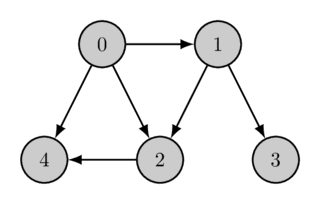
\includegraphics[width=0.35\linewidth]{img/topological_3}
	\label{fig:topological2}
\end{figure}

Un orden topológico puede \textbf{no existir} en absoluto. Solo existe si el grafo dirigido no contiene ciclos. De lo contrario porque hay una contradicción: si hay un ciclo que contiene los vértices $a$ y $b$, entonces $a$ necesita tener un índice más pequeño que $b$ (ya que puedes llegar $b$ de $a$ ) y también uno más grande (como se puede alcanzar $a$ de $b$ ). El algoritmo descrito en esta guia también muestra por construcción que cada grafo dirigido acíclico contiene al menos un orden topológico.

Para resolver este problema utilizaremos la búsqueda en profundidad (DFS). Partimos que el grafo es acíclico. ¿Qué hace la búsqueda primero en profundidad?. 

Al partir de algún vértice $v$, DFS intenta recorrer a lo largo de todas las aristas que salen de $v$. Se detiene en las aristas cuyos extremos ya han sido visitados previamente, y recorre el resto de las aristas y continúa recursivamente en sus extremos.

Por lo tanto, en el momento de la llamada a la función $\text{dfs}(v)$ ha terminado, todos los vértices que son alcanzables desde $v$ han sido visitados directamente (a través de un borde) o indirectamente por la búsqueda.

Agreguemos el vértice $v$ a una lista, cuando terminemos $\text{dfs}(v)$. Dado que ya se han visitado 
todos los vértices accesibles, ya estarán en la lista cuando agreguemos $v$. Hagamos esto para cada 
vértice del grafo, con una o varias ejecuciones de búsqueda en profundidad. Para cada arista dirigida 
$v \rightarrow u$ en el grafo, $u$ aparecerá antes en esta lista que $v$, porque $u$ es accesible desde 
$v$. Entonces, si solo etiquetamos los vértices en esta lista con $n-1, n-2, \dots, 1, 0$, hemos 
encontrado un orden topológico del grafo. En otras palabras, la lista representa el orden topológico 
inverso.

Estas explicaciones también se pueden presentar en términos de tiempos de salida del algoritmo DFS. El 
tiempo de salida para el vértice $v$ es el momento en que la función llama $\text{dfs}(v)$ terminado 
(los tiempos se pueden numerar de $0$ a $n-1$). Es fácil entender que el tiempo de salida de cualquier 
vértice $v$ siempre es mayor que el tiempo de salida de cualquier vértice accesible desde él (ya que 
fueron visitados antes de la llamada $\text{dfs}(v)$ o durante el mismo). Así, el ordenamiento 
topológico buscado son los vértices en orden decreciente de sus tiempos de salida.